\documentclass[a4paper,10pt]{article}

%linguagem
\usepackage[brazil]{babel}
%encodificação
\usepackage[utf8]{inputenc}
%biblioteca de matemática
\usepackage{amssymb,amsmath}
%pacote para codigo fonte
\usepackage{listings}
%figuras
\usepackage{graphicx}
%cores
\usepackage{color}
%paragrafo no inicio da secao
\usepackage{indentfirst}
%url
\usepackage{framed, url}
\usepackage{fancyvrb}

\usepackage{longtable}

\usepackage[table]{xcolor}
\newcommand{\p}{\cellcolor{blue}}
\usepackage{slashbox} % Linha diagonal na tabela

%define a cor "claro"
\definecolor{claro}{gray}{0.96}

%configurações do fancy verbatim
\fvset{frame=single, xleftmargin=-80pt, xrightmargin=-80pt}
%configurações do listings
\lstset{language=C,frame=trBL, numbers=left, xleftmargin=0pt, xrightmargin=0pt,breaklines=true, backgroundcolor=\color{claro}}

\begin{document}

\begin{titlepage}
\begin{center}


\includegraphics[scale=0.2]{imagens/UFMG.png}\\
\textsc{\LARGE Universidade Federal de Minas Gerais\\
	Departamento de Ciência da Computação}\\[1.5cm]

\textsc{\Large Redes de Computadores\\
	Trabalho Prático 3}\\[0.5cm]

\hrulefill \\[0.4cm]
{ \LARGE \bfseries sistema de mensagens}\\[0.4cm]

\hrulefill \\[1.5cm]
\vspace{7cm}
\begin{minipage}{0.4\textwidth}
\begin{flushleft} \large
\emph{Aluno:}\\
Pedro Araujo Pires \\
\end{flushleft}
\end{minipage}
\begin{minipage}{0.4\textwidth}
\begin{flushright} \large
\emph{Professor:}\\
Luis Felipe Menezes Vieira\\
\end{flushright}
\end{minipage}

\vfill

{\large \today}

\end{center}
\end{titlepage}


\tableofcontents
\pagebreak

\section{Introdução}

Já fazem muitos anos que não conseguimos pensar em um computador como uma
máquina isolada do mundo. As redes permitem a comunicação entre computadores, e
por consequência entre usuários. A Internet não nos deixa dúvidas.

Grande parte da comunicação entre processos é feita utilizando o modelo
cliente-servidor. Este modelo se baseia na ideia de que um processo (o cliente)
se conecta a outro (o servidor) para pedir ou enviar informações. Uma boa
analogia seria uma pessoa fazendo uma ligação telefônica para outra. A pessoa
que faz a ligação precisa de saber o número do telefone da outra, mas quem
recebe não sabe quem está ligando. Uma vez que a chamada é completada, ambas as
pessoas podem falar e/ou escutar.

\begin{figure}[ht!]
\begin{center}
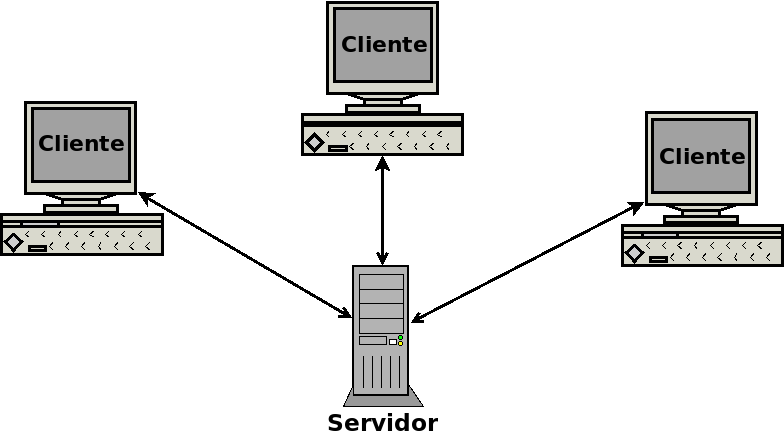
\includegraphics[scale=0.4]{imagens/clienteservidor.png}
\label{fig:clienteservidor}
\caption{Modelo cliente-servidor}
\end{center}
\end{figure}

O objetivo deste trabalho foi desenvolver uma aplicação no modelo
cliente-servidor, na qual o cliente enviava ao servidor o nome do arquivo que
desejava, e recebia este arquivo. Para isto deveria ser usada a biblioteca {\it
sockets} do Unix.

\clearpage
\section{Metodologia}

\subsection{Ambiente de testes}

Os testes feitos com {\it local host} foram realizados numa máquina com as seguintes configurações:

\begin{itemize}
\item Processador: Intel(R) Core(TM)2 Duo CPU P8600 @ 2.40GHz
\item Cache: 3072 KB
\item Memória: 3092344 KB
\item Kernel: 2.6.28-19-generic
\end{itemize}

Os testes feitos na rede do DCC/UFMG utilizaram estes recursos:

\begin{itemize}
\item Servidor:
\begin{itemize}
\item Nome na rede: tigre
\item Processador: Intel(R) Xeon(TM) CPU 2.80GHz 
\item Cache: 512 KB
\item Memória: 1025836 KB
\item Kernel: 2.6.32-22-generic
\end{itemize}

\item Cliente:
\begin{itemize}
\item Nome na rede: grande.grad
\item Processador: Intel(R) Pentium(R) 4 CPU 3.00GHz
\item Cache: 2048 KB
\item Memória: 2061260 kB
\item Kernel: 2.6.32-24-generic
\end{itemize}

\end{itemize}
\subsection{Testes}

Para medir o desempenho da aplicação foram feitos 5 tipos de testes:

\begin{table}[h!]
\centering
\begin{tabular}{|c||c|c|c|c|c|}
\hline
                   & Teste 1     & Teste 2          & Teste 3          & Teste 4          & Teste 5          \\\hline
Buffer do cliente  & $1 - 100 B$ & $2^2 - 2^{20} B$ & $2^2 - 2^{20} B$ & $256 B$          & $256 B$          \\\hline
Buffer do servidor & $256 B$     & $2^2 - 2^{20} B$ & $256 B$          & $2^2 - 2^{20} B$ & $256 B$          \\\hline
Tamanho do arquivo & $8 MB$      & $8 MB$           & $8 MB$           & $8 MB$           & $2^2 - 2^{20} B$ \\\hline
Rede               & DCC         & Local host       & Local host       & Local host       & Local host       \\\hline
\end{tabular}
\end{table}

\clearpage
\section{Resultados}

\subsection{Teste 1}

\tiny
\begin{longtable}{|c|c|c|c|c|c|c|}
\hline

Arquivo (B) & Mensagens & Cliente (B) & Servidor (B) & Throughput(B/s) & Tempo médio (s) & Desvio padrão (s) \\\hline

8388608&8388608&1&256&2062875.2&4.0744&0.176986553162 \\\hline
8388608&4194304&2&256&3569573.6&2.3548&0.105279437688 \\\hline
8388608&2796202&3&256&4966182.4&1.692&0.0687982557918 \\\hline
8388608&2097152&4&256&5518651.0&1.5236&0.0762328013391 \\\hline
8388608&1677721&5&256&6419694.0&1.3132&0.0943046128246 \\\hline
8388608&1398101&6&256&7498791.4&1.122&0.0599766621279 \\\hline
8388608&1198372&7&256&8392172.8&1.002&0.0495015151283 \\\hline
8388608&1048576&8&256&9277943.4&0.9066&0.0468299049753 \\\hline
8388608&932067&9&256&10079842.6&0.837&0.0623153271676 \\\hline
8388608&838860&10&256&11085743.0&0.7634&0.0731754057044 \\\hline
8388608&762600&11&256&12588262.2&0.67&0.0517609891714 \\\hline
8388608&699050&12&256&12332047.2&0.6834&0.0451158508731 \\\hline
8388608&645277&13&256&12230593.2&0.6896&0.0494271180629 \\\hline
8388608&599186&14&256&13313152.6&0.6348&0.0527575587002 \\\hline
8388608&559240&15&256&13456601.4&0.6308&0.0676739240772 \\\hline
8388608&524288&16&256&15032842.0&0.5672&0.0698638676284 \\\hline
8388608&493447&17&256&13859287.4&0.6096&0.0479691567572 \\\hline
8388608&466033&18&256&15122386.8&0.5608&0.0563858138187 \\\hline
8388608&441505&19&256&14892731.4&0.5694&0.0624070508837 \\\hline
8388608&419430&20&256&14586653.8&0.5794&0.0537311827527 \\\hline

\end{longtable}

\begin{longtable}{|c|c|c|c|c|c|c|}
\hline

Arquivo (B) & Mensagens & Cliente (B) & Servidor (B) & Throughput(B/s) & Tempo médio (s) & Desvio padrão (s) \\\hline

8388608&8388608&1&256&667809.6&12.5628&0.133760083732 \\\hline
8388608&4194304&2&256&1226222.6&6.845&0.168712773672 \\\hline
8388608&2796202&3&256&1750218.0&4.7938&0.0733332121211 \\\hline
8388608&2097152&4&256&2109493.2&3.9776&0.0627075753 \\\hline
8388608&1677721&5&256&2416793.8&3.4796&0.18060852693 \\\hline
8388608&1398101&6&256&2829486.0&2.965&0.0340998533721 \\\hline
8388608&1198372&7&256&3055965.8&2.7498&0.114705536048 \\\hline
8388608&1048576&8&256&3458621.8&2.4362&0.169287211567 \\\hline
8388608&932067&9&256&3537819.2&2.3918&0.231379687959 \\\hline
8388608&838860&10&256&3966290.4&2.1156&0.0367347247165 \\\hline
8388608&762600&11&256&4017549.8&2.1082&0.221633390986 \\\hline
8388608&699050&12&256&4007006.2&2.1208&0.246909214085 \\\hline
8388608&645277&13&256&4495012.0&1.8692&0.0728900541912 \\\hline
8388608&599186&14&256&4599391.8&1.8418&0.194643674441 \\\hline
8388608&559240&15&256&4761727.6&1.7664&0.0941352218885 \\\hline
8388608&524288&16&256&5031701.0&1.6692&0.0592330988553 \\\hline
8388608&493447&17&256&5027089.2&1.6826&0.1641396966 \\\hline
8388608&466033&18&256&5454700.0&1.538&0.0242074368738 \\\hline
8388608&441505&19&256&5235548.2&1.6496&0.316897838427 \\\hline
8388608&419430&20&256&5385718.2&1.587&0.238596730908 \\\hline
\end{longtable}

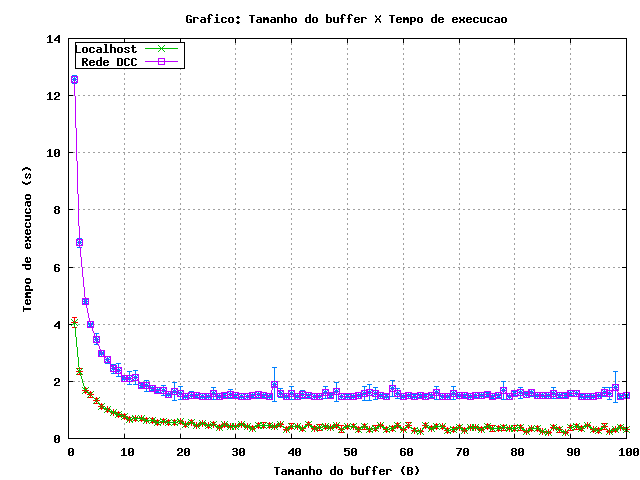
\includegraphics[scale=0.5]{imagens/teste1.png}

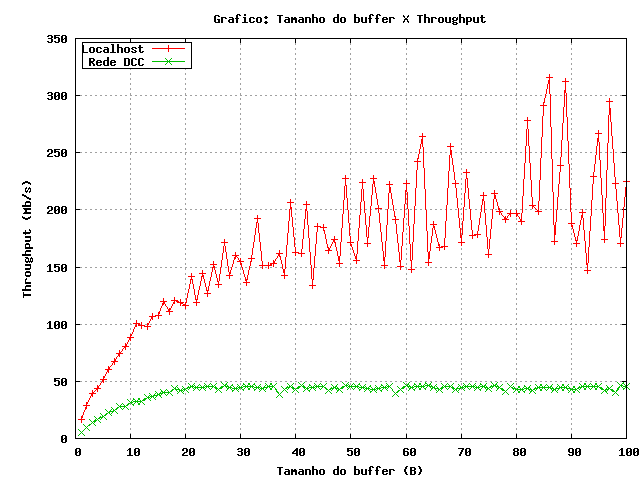
\includegraphics[scale=0.5]{imagens/teste1-2.png}

\clearpage
\subsection{Teste 2}
\tiny
\begin{longtable}{|c|c|c|c|c|c|c|}
\hline

Arquivo (B) & Mensagens & Cliente (B) & Servidor (B) & Throughput(B/s) & Tempo médio (s) & Desvio padrão (s) \\\hline

8388608&8388608&1&1&1657323.4&5.0658&0.149301574004 \\\hline
8388608&4194304&2&2&3331501.8&2.5192&0.0557329346078 \\\hline
8388608&2097152&4&4&5451350.8&1.5442&0.0914885785221 \\\hline
8388608&1048576&8&8&11632143.8&0.722&0.0250758848299 \\\hline
8388608&524288&16&16&19309100.0&0.4368&0.0324678302324 \\\hline
8388608&262144&32&32&26990873.8&0.327&0.0782483226657 \\\hline
8388608&131072&64&64&35181053.0&0.2484&0.0469748869078 \\\hline
8388608&65536&128&128&47078314.0&0.1962&0.07342315711 \\\hline
8388608&32768&256&256&59563300.4&0.1458&0.0271322686114 \\\hline
8388608&16384&512&512&66050800.6&0.139&0.043717273474 \\\hline
8388608&8192&1024&1024&58031397.2&0.1592&0.0513513388336 \\\hline
8388608&4096&2048&2048&54281358.6&0.1552&0.00915204895092 \\\hline
8388608&2048&4096&4096&74166987.0&0.1204&0.0283873211135 \\\hline
8388608&1024&8192&8192&86785310.4&0.1164&0.0364614865303 \\\hline
8388608&512&16384&16384&72123437.6&0.1338&0.0425835649048 \\\hline
8388608&256&32768&32768&62608057.0&0.14&0.0286775173263 \\\hline
8388608&128&65536&65536&70170422.0&0.1238&0.0218027521199 \\\hline
8388608&64&131072&131072&84908286.8&0.1164&0.0407214930964 \\\hline
8388608&32&262144&262144&59113112.4&0.1444&0.0187040102652 \\\hline
8388608&16&524288&524288&79570291.2&0.1186&0.0377920626587 \\\hline

\end{longtable}

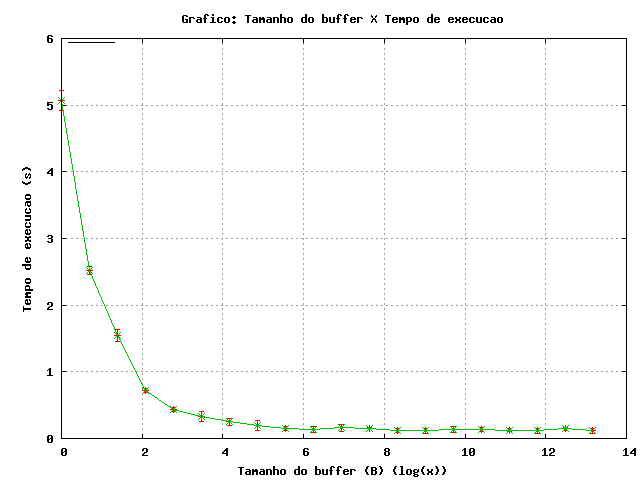
\includegraphics[scale=0.5]{imagens/teste2.png}

\clearpage
\subsection{Teste 3}

\tiny
\begin{longtable}{|c|c|c|c|c|c|c|}
\hline

Arquivo (B) & Mensagens & Cliente (B) & Servidor (B) & Throughput(B/s) & Tempo médio (s) & Desvio padrão (s) \\\hline

8388608&8388608&1&256&1968625.4&4.2716&0.210337443172 \\\hline
8388608&4194304&2&256&3529079.0&2.3862&0.145882692599 \\\hline
8388608&2097152&4&256&5430882.6&1.5488&0.0838579751723 \\\hline
8388608&1048576&8&256&9333127.0&0.9006&0.0387329317248 \\\hline
8388608&524288&16&256&13669056.4&0.618&0.0519730699497 \\\hline
8388608&262144&32&256&17389012.6&0.4924&0.0688668280088 \\\hline
8388608&131072&64&256&27518235.8&0.3124&0.0461891762213 \\\hline
8388608&65536&128&256&50810993.4&0.187&0.0600965889215 \\\hline
8388608&32768&256&256&24754989.0&0.3518&0.0709799971823 \\\hline
8388608&16384&512&256&26753826.2&0.3232&0.0544147038952 \\\hline
8388608&8192&1024&256&34630760.6&0.2576&0.0681222430635 \\\hline
8388608&4096&2048&256&34734743.8&0.2766&0.108197227321 \\\hline
8388608&2048&4096&256&27659035.4&0.3142&0.0524038166549 \\\hline
8388608&1024&8192&256&39353828.4&0.2156&0.0232860473245 \\\hline
8388608&512&16384&256&37149975.8&0.2288&0.0275056357861 \\\hline
8388608&256&32768&256&24178138.0&0.3504&0.0343953485227 \\\hline
8388608&128&65536&256&27341616.8&0.3102&0.0317578336793 \\\hline
8388608&64&131072&256&38896749.6&0.2512&0.11845741851 \\\hline
8388608&32&262144&256&30262570.6&0.2896&0.0644440842902 \\\hline
8388608&16&524288&256&29114682.8&0.2934&0.0390107677443 \\\hline

\end{longtable}

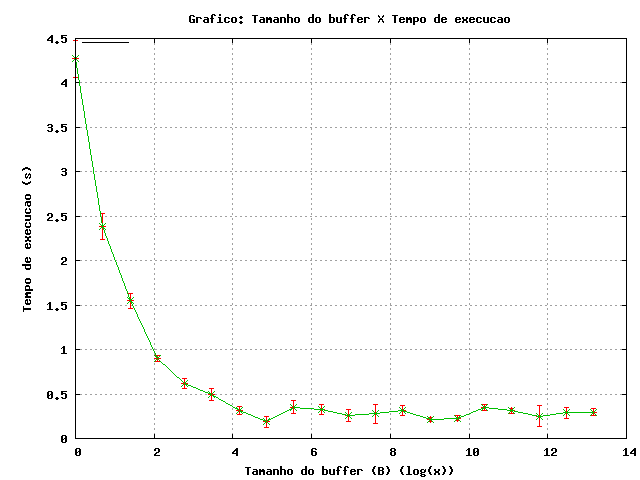
\includegraphics[scale=0.5]{imagens/teste3.png}

\clearpage
\subsection{Teste 4}

\tiny
\begin{longtable}{|c|c|c|c|c|c|c|}
\hline

Arquivo (B) & Mensagens & Cliente (B) & Servidor (B) & Throughput(B/s) & Tempo médio (s) & Desvio padrão (s) \\\hline

8388608&32768&256&1&815032.4&10.6578&2.08257325441 \\\hline
8388608&32768&256&2&1437585.8&6.3418&2.10661314911 \\\hline
8388608&32768&256&4&3274157.0&2.5922&0.283432813908 \\\hline
8388608&32768&256&8&7512451.4&1.1266&0.110280732678 \\\hline
8388608&32768&256&16&13513762.4&0.6294&0.072145963158 \\\hline
8388608&32768&256&32&23695162.2&0.3654&0.0657741590596 \\\hline
8388608&32768&256&64&31177458.0&0.2786&0.0524846644269 \\\hline
8388608&32768&256&128&55996099.8&0.1508&0.0121720992438 \\\hline
8388608&32768&256&256&64617772.0&0.141&0.0434741302386 \\\hline
8388608&32768&256&512&57891420.4&0.1462&0.0135262707351 \\\hline
8388608&32768&256&1024&66481575.4&0.1374&0.032616560211 \\\hline
8388608&32768&256&2048&57807662.6&0.1534&0.0328060969943 \\\hline
8388608&32768&256&4096&64766461.2&0.1576&0.0581639063337 \\\hline
8388608&32768&256&8192&52784695.6&0.1684&0.0399629828717 \\\hline
8388608&32768&256&16384&65822681.8&0.1428&0.0400519662439 \\\hline
8388608&32768&256&32768&49995110.8&0.1716&0.025112546665 \\\hline
8388608&32768&256&65536&52123089.8&0.166&0.030698534167 \\\hline
8388608&32768&256&131072&64863916.0&0.151&0.0466047207909 \\\hline
8388608&32768&256&262144&47770527.6&0.1806&0.0307935058089 \\\hline
8388608&32768&256&524288&62283691.0&0.1488&0.0412232943856 \\\hline

\end{longtable}

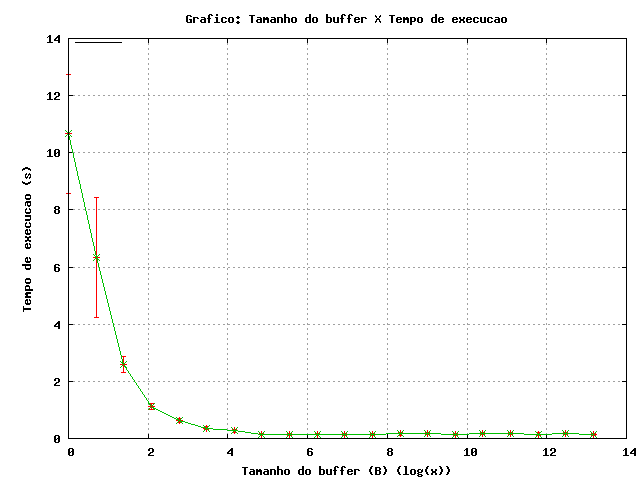
\includegraphics[scale=0.5]{imagens/teste4.png}

\clearpage
\subsection{Teste 5}

\tiny
\begin{longtable}{|c|c|c|c|c|c|c|}
\hline

Arquivo (B) & Mensagens & Cliente (B) & Servidor (B) & Throughput(B/s) & Tempo médio (s) & Desvio padrão (s) \\\hline

4&0&256&256&2780.2&0.0074&0.00868562030024 \\\hline
8&0&256&256&11581.6&0.0014&0.00135646599663 \\\hline
16&0&256&256&34879.6&0.0004&0.000489897948557 \\\hline
32&0&256&256&43607.4&0.001&0.000632455532034 \\\hline
64&0&256&256&171321.0&0.0002&0.0004 \\\hline
128&0&256&256&351144.6&0.0002&0.0004 \\\hline
256&1&256&256&494253.4&0.0004&0.000489897948557 \\\hline
512&2&256&256&1340839.0&0.0002&0.0004 \\\hline
1024&4&256&256&2103045.8&0.0004&0.000489897948557 \\\hline
2048&8&256&256&4300130.8&0.0004&0.000489897948557 \\\hline
4096&16&256&256&10321776.2&0.0004&0.000489897948557 \\\hline
8192&32&256&256&18490989.8&0.0006&0.000489897948557 \\\hline
16384&64&256&256&24337550.6&0.0042&0.00691086101727 \\\hline
32768&128&256&256&40721008.8&0.001&0.0 \\\hline
65536&256&256&256&43902391.4&0.0046&0.0058172158289 \\\hline
131072&512&256&256&57666371.2&0.0026&0.0008 \\\hline
262144&1024&256&256&54712829.2&0.0076&0.00585149553533 \\\hline
524288&2048&256&256&69807231.0&0.0078&0.00116619037897 \\\hline
1048576&4096&256&256&58772768.4&0.0378&0.0456306914258 \\\hline
2097152&8192&256&256&27323167.0&0.0892&0.0382852451997 \\\hline
4194304&16384&256&256&57146309.0&0.089&0.045615786741 \\\hline
8388608&32768&256&256&60822113.0&0.2538&0.161603712829 \\\hline
16777216&65536&256&256&84595810.8&0.3386&0.190624867213 \\\hline
33554432&131072&256&256&56160140.8&0.696&0.238463414385 \\\hline
67108864&262144&256&256&55934939.2&1.3972&0.4062764576 \\\hline

\end{longtable}

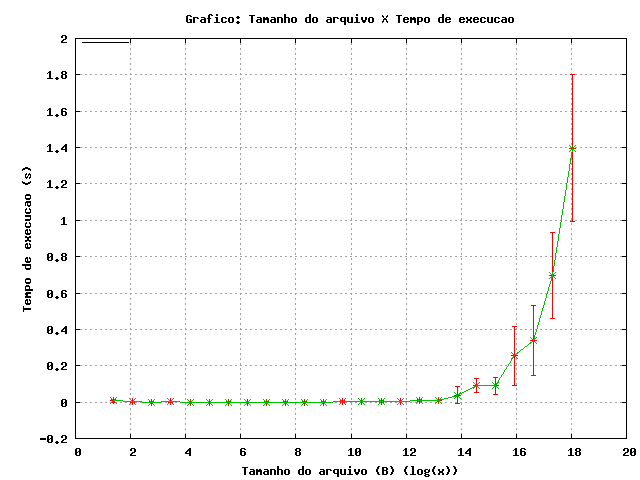
\includegraphics[scale=0.5]{imagens/teste5.png}

\normalsize

\clearpage
\section{Análise dos resultados}

O primeiro teste compara o desempenho do programa para diferentes tamanhos de
buffer do cliente, na mesma máquina e em máquinas diferentes. Podemos notar no
primeiro gráfico que o tempo de execução cai de forma exponencial em relação ao
crescimento do tamanho do buffer até se estabilizar a partir de tamanhos de
buffer acima de 10 bytes. Isto ocorre pois quanto menor o tamanho do buffer,
mais mensagens tem que ser enviadas para transferir o arquivo. A cada mensagem
enviada existe um overhead para acessar a memória, e realizar trocas de contexto
no sistema operacional. Nos casos com tamanho de buffer maior que 10 bytes o
overhead passa a ser insignificante, pois o número de mensagens é bem menor.
Nestes casos o tempo de execução depende apenas da velocidade de cópia entre o
servidor e o cliente. Isto explica a diferença entre o ambiente de testes na
mesma máquina e o ambiente em duas máquinas diferentes. No primeiro ambiente o
throughput não é limitado pela rede, portanto a velocidade de cópia é mais alta.
O segundo gráfico mostra que o throughput do segundo ambiente não passa de cerca
de 40 Mb/s, pois a rede não permite uma vazão de dados maior.

Os testes 2,3 e 4 mostram que o aumento do tamanho do buffer tanto do cliente
quanto do servidor resultam em um tempo de execução menor. A variação dos
buffers do cliente e do servidor tem efeitos semelhantes. A combinação dos dois
que vai determinar o tempo de execução. Quando o buffer do servidor é muito
pequeno, o servidor envia o arquivo em pedaços muito granulares. De forma análoga
quando o tamanho do buffer do cliente é pequeno, o cliente só consegue receber
pedaços reduzidos do arquivo.

O teste 5 revela uma situação natural. Quanto maior o arquivo a ser transferido,
mais tempo demora para ocorrer a transação.

\clearpage
\section{Conclusão}

O desenvolvimento deste trabalho possibilitou o aprendizado acerca do
funcionamento do protocolo TCP. Pudemos aprender como funciona a biblioteca
{\it sockets} do Unix e através dela fomos capazes de gerar o um programa no
modelo cliente-servidor

O desenvolvimento desse trabalho foi muito importante para consolidar a matéria
vista em sala de aula e colocar em prática a teoria por trás das redes de
computadores.

\clearpage
\begin{thebibliography}{99}
\bibitem{howto} \url{http://www.linuxhowtos.org/C_C++/socket.htm}
\bibitem{slide} \url{http://www.slideshare.net/jignesh/socket-programming-tutorial}
\end{thebibliography}

\end{document}
